\section{Introduction}\label{sec:intro}

The Clay problem asks for a nontrivial quantum Yang--Mills theory on
$\R^4$ for every compact simple gauge group, with Hamiltonian spectrum
in $\{0\}\cup[\Delta,\infty)$ for some $\Delta>0$ \cite{JW06}.
In a Euclidean construction the gauge-invariant Schwinger functions must
satisfy reconstruction axioms \cite{OS73,OS75}. A gap then bounds the
decay of vacuum-subtracted time correlations by $e^{-\Delta t}$ for
observables creating finite-norm states. We use Wilson's lattice theory
\cite{Wil74}: an element $Q_e$ of $G\subset\U(N)$ sits on every link $e$ of the
lattice $a\Z^4$, and a configuration has the weight
$\exp(N\beta\sum_p\ReTr Q_p)$, where $Q_p$ is the ordered product around the
plaquette~$p$.\footnote{This is the normalisation of~\cite{SZZ23}. The
conventional inverse coupling is $\beta_W=N^2\beta$, and for $\SU(2)$,
identified with the unit quaternions, $\beta_W=4\beta$.} Asymptotic freedom
forces the continuum limit $a\to0$ to be taken with $\beta\to\infty$, that is,
at weak coupling.

At small $\beta$ the lattice theory has a unique state, exponential clustering
and a transfer-matrix gap, by convergent expansions \cite{OSei78,Sei82};
Ba{\l}aban's renormalisation group \cite{Bal84a,Bal85a,Bal89b} gives ultraviolet
stability in finite volume at weak coupling (Dimock \cite{Dim13} presents the
method for the scalar $\phi^4$ model in three dimensions), and Magnen, Rivasseau and S\'en\'eor constructed the theory with an
infrared cutoff \cite{MRS93}. No existing result gives a mass gap in physical
units for the four-dimensional continuum theory of the Clay problem.
We prove a strong-coupling lattice gap for every compact simple group.
For isotropic $\SU(2)$ we compute the weak-coupling gap on a fixed free
cube (Theorem~\ref{thm:isotropic-free-box}). On growing boxes,
Theorem~\ref{cl:thm:exterior-mean-curvature} controls the average Wilson
plaquette deficit for every exterior field. Reaching the continuum gap
would require a physical-scale correlation estimate in addition to this
control of the local action.


\noindent\emph{Unequal Wilson couplings.}\enspace
When the spatial and temporal plaquette coefficients are varied separately,
the partition functions admit a direct estimate.
Theorem~\ref{cl:thm:unequal-gap} gives a gap in the gauge-invariant
transfer spectrum uniformly in spatial volume. For $\SU(2)$ it also
allows time to become continuous with a nonzero spatial interaction.
Theorem~\ref{cl:thm:electric-packet} bounds a plaquette correlation
from above and below in that limit. The spatial cutoff remains fixed.

\subsection{The single-cube criterion}
Sections~\ref{sc:sec:psts}--\ref{sc:sec:continuum}
give a sharper one-scale criterion: one cube of spatial side $2T_0$ and
time extent $T_0$ suffices, through the cutoff-free inequality
\[
2\log Z((2T_0)^3,T_0)-\log Z((2T_0)^3,2T_0)\le\frac1{4097}.
\]
If this holds at the actual tuned Wilson couplings with $3\le T_0\le Nt_0$,
the compatible continuum theory has gap at least
$t_0^{-1}\log(63/32)$. Purity conversion, an exchange of lattice directions
and a nonlinear ascent prove this implication without assuming a gap on
the starting cube. They do not prove the displayed inequality at weak
coupling.

The distinction between the theorem and its inputs is essential. Strong
coupling proves a lattice theory in a stated coupling range. The
criterion is valid, conditionally, for each compact gauge group with the
required positive transfer structure. Neither the criterion nor the code
proves its weak-coupling input, constructs nontrivial continuum observables,
or settles the additional flux-sector issues for quotient groups. The
status of the Clay requirements is stated explicitly in
Section~\ref{sc:ssec:clay}.

The Wilson measure itself enters the exact constructions of
Sections~\ref{cl:sec:replica}--\ref{cl:sec:retention}. Two replica cuts
express the cube datum as a signed connected response with an explicit
threshold. A conditional trace factorisation identifies the appropriate
tilted histories. A frustrated central-link field gives a quantitative
obstruction to a global pointwise kernel certificate, while the exact
Wilson Dirichlet form separates retention of a physical excitation from
a lower spectral gap. These identities specify the remaining estimates
without replacing them by independence or a Gaussian approximation.


Section~\ref{cl:sec:fisher} proves that every one-link prefix conditional
of the Wilson vacuum has Poincar\'e constant at most $e^{12b}/3$, independent
of spatial volume. It turns the thermal trace estimate into a bound on
conditional transition scores under squared-likelihood tilted histories.
The conditional comparison includes large fields; the required decay of
those scores along the tuning remains unproved. Proposition~\ref{cl:prop:spectral-mass}
also characterises retention by bounded-energy spectral mass, without
requiring an energy upper bound on the whole unfiltered observable.
Appendix~\ref{cl:app:flow} supplies a support-preserving regularisation
and quantifies the errors that such an observable construction must control.

\subsection{The lattice gap with explicit constants}

Let $G$ be a compact connected Lie group with semisimple Lie algebra,
identified with its image under a faithful unitary representation in $\U(N)$,
and let $\kappa_G>0$ be its least Ricci curvature for the bi-invariant metric
$\ip XY=-\Tr(XY)$. For a simple group $\kappa_G=h^\vee/(2\ell_\rho)$, with $h^\vee$
the dual Coxeter number and $\ell_\rho$ the Dynkin index of the representation;
for $\SU(N)$, $\kappa_G=N/2$.\footnote{For a bi-invariant metric on a compact
Lie group the Ricci curvature is $\operatorname{Ric}(X,X)=-\frac14B(X,X)$
with $B$ the Killing form, $B(X,Y)=\Tr(\operatorname{ad}_X\operatorname{ad}_Y)$.
For $\mathfrak{su}(N)$, $B(X,Y)=2N\Tr(XY)$, so $\operatorname{Ric}(X,X)=
\frac N2\,\ip XX$ in the metric $\ip XY=-\Tr(XY)$ of the defining
representation, which is the value $\kappa_G=N/2$; in general the Killing form
is $2h^\vee$ times the trace form of the adjoint representation and
$2\ell_\rho$ times that of $\rho$, which gives $h^\vee/(2\ell_\rho)$.}

\begin{mainthm}\label{thm:A}
Suppose $N|\beta|<\frac2{29}\kappa_G$. For every gauge-invariant local
observable the expectations in boxes with free boundary converge, along every
exhausting sequence of boxes, to a state $\omega$ that is invariant under the
lattice symmetries; truncated correlations of Lipschitz observables decay at
every rate below
\[
m_G(\beta)=\operatorname{arccosh}\Bigl(1+\frac1{12}\Bigl(\frac{\kappa_G}{N|\beta|}
-\frac{29}2\Bigr)\Bigr)>0 ,
\]
and for $\beta\ge0$ the state is reflection positive and its transfer matrix
has spectral gap $m\ge m_G(\beta)$. For $G=\SU(2)$ the clustering statement holds for
$|\beta_W|<\frac13$; for $0\le\beta_W<\frac13$ the reflection-positive
transfer matrix satisfies $m\ge-\log(3\beta_W)$, with $-\log0=+\infty$.
\end{mainthm}

Two ingredients carry the proof. The first is a gauge: a field of straight
lines on $\Z^4$ that contains exactly one link of every plaquette
(Sec.~\ref{sec:linefield}). Setting these links to the identity loses no
gauge-invariant information, and every remaining link then interacts with
exactly twelve others instead of eighteen. The second is a Hessian bound in
this gauge, $|\Hess S|\le\frac{29}2$ for the action $S=\sum_p\ReTr Q_p$, proved
by a divergence identity and a positivity statement for one plaquette
(Sec.~\ref{sec:curvature}); with the Ricci curvature of $G$ it gives a
Bakry--\'Emery bound \cite{BE85,BGL14} with an explicit decay rate. Without
the gauge no Bakry--\'Emery constant is positive beyond $|\beta_W|=N^2/32$
(Theorem~\ref{thm:fullspace}), so the gauge enlarges the range of every group
by the factor $32/29$ and supplies the rate. The $\SU(2)$ statement combines
the gauge with the sharp Kantorovich modulus $\frac14$ of the von
Mises--Fisher family, proved in Appendix~\ref{app:sharp}, in Dobrushin's
criterion \cite{Dob68,Dob70}.

\subsection{A continuum mass gap from one cube}

The lattice gap of Theorem~\ref{thm:A} is measured in lattice units. A fixed positive lattice gap would diverge in physical units as $a\to0$; the issue for Yang--Mills is that the theorem does not cover the required tuning $\beta\to\infty$. The second result isolates a single
estimate, posed on one scale, that controls the gap in physical units. On a
periodic lattice let $\mathcal P_x$ resample the links of the cube of side $n$
at $x$ from their conditional law under the Wilson measure $\mu$. The
condition $\BP(n,\varpi)$ asks that
\[
\varpi\Var_\mu(f)\le\frac1{n^4}\sum_x\mu\bigl((f-\mathcal P_xf)^2\bigr)
\]
for every gauge-invariant $f$: the dynamics that resamples cubes, each link
at rate one, has spectral gap at least $\varpi$ on gauge-invariant functions.
The condition involves no gauge fixing and no supremum over boundary
conditions.

\begin{mainthm}\label{thm:B}
Let $a_k\to0$ and $\beta_k\ge0$ be couplings, and suppose that there are
$\varpi>0$, $\ell>0$ and integers $n_k\ge2$ with $n_ka_k\le\ell$ such that
$\BP(n_k,\varpi)$ holds for the Wilson measure at $\beta_k$ on all large tori.
Then every continuum limit of the corresponding lattice theories has
Hamiltonian $H$ with $\sigma(H)\subset\{0\}\cup[\Delta,\infty)$,
\[
\Delta=\frac{16\varpi}{625e^2\ell},
\]
and $0$ is a simple eigenvalue; if the limit is nontrivial, $H$ has a mass
gap of at least $\Delta$.\footnote{The constant comes from the finite-speed
bound: the cube chain decorrelates two observables at lattice distance $s$
at the rate $\varpi/(e^2q_nn)$ per unit of $s$, where $q_n=(2+1/n)^4$ is the
number of cubes of side $n$ that meet a given one, divided by $n^4$;
$q_n\le(5/2)^4=625/16$ for $n\ge2$, and $na\le\ell$ converts the lattice rate
into the physical rate $\varpi/(e^2q_n\,na)\ge16\varpi/(625e^2\ell)$. The
factor $e^2$ is the loss in the Poisson tail estimate of Lemma~\ref{lem:speed}.}
\end{mainthm}

The proof (Sec.~\ref{sec:cube}) turns the spectral gap into decay of
covariances through a finite-speed bound for the cube dynamics, at a rate
of order $1/n$ in lattice units, hence of order $1/\ell$ in physical units,
and passes this decay through the Osterwalder--Schrader reconstruction.

\begin{figure}[t]
\centering
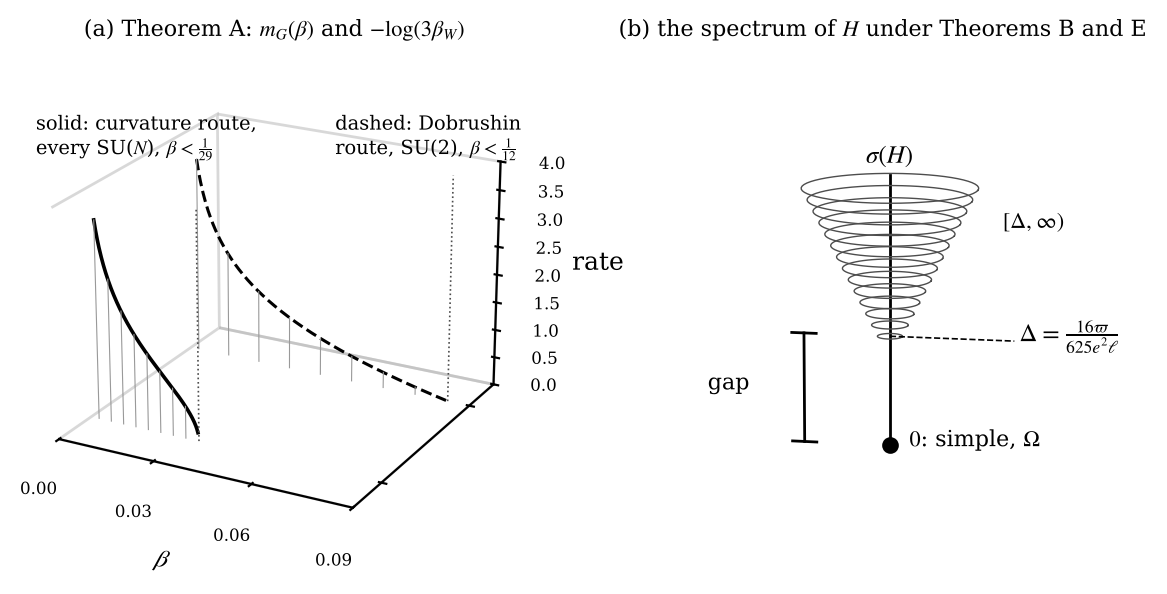
\includegraphics[width=\textwidth]{figures/fig_spectrum.png}
\caption{(a) The rates of Theorem~\ref{thm:A}: the curvature route gives $m_G(\beta)=\operatorname{arccosh}\bigl(1+\frac1{12}(\frac{\kappa_G}{N|\beta|}-\frac{29}2)\bigr)$ for $N|\beta|<\frac2{29}\kappa_G$, which for every $\SU(N)$, where $\kappa_G=N/2$, is the one curve drawn for $\beta<\frac1{29}$; the Dobrushin route for $\SU(2)$ gives $-\log(3\beta_W)=-\log(12\beta)$ for $\beta<\frac1{12}$. (b) The spectrum of the Hamiltonian under Theorems~\ref{thm:B} and~\ref{thm:E}: $0$ is a simple eigenvalue with eigenvector $\Omega$, and the rest of the spectrum lies in $[\Delta,\infty)$ with $\Delta=16\varpi/(625e^2\ell)$.}
\label{fig:spectrum}
\end{figure}

\subsection{The theories constructed on tori}

Theorem~\ref{thm:B} takes the lattice theory to infinite volume before the
lattice spacing is sent to zero. A continuum theory may also be
built in the opposite order: at a fixed physical side $L_p$ of a symmetric
torus the mesh $a_N=1/N$ is sent to zero, with couplings $\beta_{N,p}$, and the
side is sent to infinity afterwards. Section~\ref{sec:bridge} considers any
such construction whose outcome is a mixture, over a compact space $X$ of
phases carrying a measure $\nu$ of full support, of theories $S^\chi$ each
satisfying the Wightman axioms with a unique vacuum; this is hypothesis (W),
stated in full in Definition~\ref{def:WUD}; it is the shape of the
conclusion claimed by the unrefereed Lean~4 construction~\cite{OAI26,YMG26},
on which nothing below depends. At finite side the lattice state
is a thermal state at temperature $1/L_p$, and a decay estimate for its
two-point functions is not what a gap controls, so a gap for such a theory
needs more than (D). Call (U) the hypothesis that the same limit is obtained when the Euclidean time
extent of the torus is sent to infinity first, at each mesh, and
(D$_\ell$) the cube condition $\BP(n_N,\varpi)$ with $n_Na_N\le\ell$ on all
cylinders $(\Z/NL_p\Z)^3\times(\Z/M\Z)$, $M\ge2n_N+4$, at the couplings
$\beta_{N,p}$ of the construction.

\begin{mainthmE}
Under \textup{(W)}, \textup{(U)} and \textup{(D$_\ell$)} the phases $S^\chi$
all coincide, and the Wightman theory of the construction has Hamiltonian
$H$ with $\sigma(H)\subset\{0\}\cup[\Delta,\infty)$, $\Delta=16\varpi/(625e^2
\ell)$, and $0$ a simple eigenvalue.
\end{mainthmE}

This is Theorem~\ref{thm:E}; it is a theorem about the three hypotheses, and
it rests on nothing outside this paper. Two of the hypotheses can be
weakened: (U) may be replaced by the single renormalisation-free statement
(Z) that the partition function of the symmetric torus, divided by the
$NL_p$-th power of the leading eigenvalue of the transfer matrix of the
cylinder of the same side, tends to $1$ (Corollary~\ref{cor:Z}, through a
sharp inequality bounding the thermal correction of any slab observable by
that quantity, Lemma~\ref{lem:thermaldiscrepancy}); and (D$_\ell$) follows
from the slab decorrelation of Theorem~\ref{thm:D} at one physical
separation, since that theorem holds on cylinders
(Corollary~\ref{cor:cylinders}, Proposition~\ref{prop:bridgeM}). Its proof builds the transfer matrix of a
cylinder as a positive integral operator with a strictly positive kernel on
the gauge-invariant slice functions, deduces from the cube condition a gap of
the cylinder's zero-temperature Hamiltonian, carries the decay of the
renormalised two-point functions through the two limits with a constant that
depends only on the test functions, and identifies the limit of the Euclidean
vectors of the lattice theories with the vectors of the Wightman theory; the
triviality of the phase decomposition is a consequence of the same decay.
What Theorem~\ref{thm:E} does not do is prove (D$_\ell$): along the tuning of
the construction the coupling tends to infinity, and the cube condition at
weak coupling is exactly statement (D) of Sec.~\ref{sec:remains}.

\subsection{One bound at one scale}

The hypotheses of Theorem~E can be replaced by a single one that mentions
neither cubes, nor slabs, nor a gap. For a spatial torus $s$ with sides
$s_1,s_2,s_3$ and volume $V(s)$ let $\mathcal Z_s(T)$ be the partition
function of the torus $s\times(\Z/T\Z)$ divided by the $T$-th power of the
leading eigenvalue of the transfer matrix of $s$; it is the trace of the
$T$-th power of the normalised transfer matrix, and $\log\mathcal Z_s(T)$ is
the thermal part of the free energy at inverse temperature $T$. Hypothesis
(B$^{*}$) asks that, at one time extent $T_0$ of a fixed physical size,
\[
\log\mathcal Z_s(T_0)\le\gamma V(s),\qquad 2\gamma(96T_0)^3\le\tfrac1{20},
\]
for the spatial tori whose sides lie between $2T_0$ and $48T_0$.

\begin{mainthmF}
Under \textup{(W)} and \textup{(B$^{*}$)} at one physical time extent $t_0$,
the phases $S^\chi$ coincide and the Wightman theory of the construction has
$\sigma(H)\subset\{0\}\cup[\Delta,\infty)$ with $0$ a simple eigenvalue and
$\Delta\ge0.172/t_0$.
\end{mainthmF}

The full statement is in Section~\ref{ssec:onehyp}. Its proof doubles the
time extent: positivity of the transfer matrix and the exchange of the four
directions of the torus turn the bound at $T_0$ into a smaller bound at
$2T_0$ on a wider family of tori, and the iteration, which decreases doubly
exponentially, produces the gap of every large torus together with~(Z)
(Figure~\ref{fig:ascent}). The hypothesis is equivalent, up to a factor two in $\gamma$, to a finite
inequality between two partition functions,
$Z(s,T_0)^2\le e^{\gamma V(s)}Z(s,2T_0)$, in which no eigenvalue appears
(Proposition~\ref{prop:Bfinite}). It is not proved here at weak coupling,
and it cannot be easy: it contains the lattice mass gap at the scale $T_0$
(Proposition~\ref{prop:Bhard}), and for $\SU(2)$ the gap of a torus of fixed
lattice size closes as the coupling grows (Theorem~\ref{thm:gapcloses}), so
that $T_0$ must grow along the tuning (Corollary~\ref{cor:basescale}).
Appendix~\ref{app:degenerate} shows that the shortcuts which avoid the
renormalised theory, among them the limit of the parallel transporters
themselves, lead to trivial theories (Theorem~\ref{thm:haarlimit},
Proposition~\ref{prop:planar}).

\subsection{Where the cube condition holds}

\begin{mainthm}\label{thm:C}
\begin{enumerate}[label=\textup{(\roman*)},leftmargin=*]
\item At $\beta=0$, $\BP(n,1)$ holds for every $n$. For
$21N|\beta|<\kappa_G$ and $n$ large, $\BP(n,1-\alpha_n)$ holds with
$\alpha_n=N|\beta|(18n-3)/((\kappa_G-21N|\beta|)n^2)\to0$; for $\SU(2)$ the
range is $|\beta_W|<\frac5{18}$, and for $\SU(3)$ it contains
$0\le\beta_W\le0.45$.
\item For the free scalar field of lattice mass $\mu$ in $d$ dimensions the
best constant is
$\varpi=\frac{\mu^2}{n^d}\ip{\mathbf 1}{(-\Delta_D+\mu^2)^{-1}\mathbf 1}$, with
$-\Delta_D$ the Dirichlet Laplacian of the cube, and with $s=n\mu$ (the mass
times the physical size of the cube)
\[
\Bigl(\frac56\Bigr)^d\frac{s^2}{s^2+10d}\le\varpi\le\frac{s^2}{s^2+16d/9}.
\]
\item For $G=\SU(2)$ and $|\beta_W|\le\frac7{20}$, $\BP(n,\varpi)$ holds for
every $n\ge2$ with $\varpi=\frac{106}{1933}\cdot517^{-4}$, independent of $n$
and of the torus, and $\BP(n,1-259/n)$ holds for $n\ge260$. For
$0\le\beta_W\le\frac9{25}$ every torus limit is reflection positive and its
transfer matrix has spectral gap at least $7/(625\cdot2957\,e^2)$.
\end{enumerate}
\end{mainthm}

Part (ii) is the model case of the continuum tuning: the constant is uniform
in the lattice spacing at fixed $m\ell$, and it vanishes as $m\to0$. The cube
condition is therefore a quantitative statement of mass generation at the
scale $\ell$. Part (i) is proved in Sec.~\ref{sec:bpstrong} by the gauge of
Theorem~\ref{thm:A} and a weighted Dobrushin criterion for blocks of links.
No argument built on single-link updates in this gauge passes
$\beta_W=\frac13$ for $\SU(2)$ (Proposition~\ref{prop:methodlimit}). Part
(iii) passes that value by resampling \emph{stars}, the eight links at a
vertex of one parity (Sec.~\ref{sec:stars}): the perturbation of one
plaquette at a vertex enters the law of a star only through the relative
variable of two of its links, and no plaquette is internal to a star.

\subsection{Mass generation at one scale}

Statement (D) below asks for the cube condition along the continuum tuning.
Section~\ref{sec:massgen} reduces it to a hypothesis of a different kind,
closer to physics. Split a box of the lattice, all of whose widths lie
between $2d-1$ and $md-1$, into two outer parts of width $d$ and a middle of
width $d-1$ in one coordinate, fix an arbitrary configuration outside the
box, and let $\rho$ be the maximal correlation between the gauge-invariant
observables of the two outer parts under the conditional law. The hypothesis
$(\mathrm M_{d,m}(c))$ asks that $\rho\le c$ for all such boxes, splittings
and boundary conditions. Along the tuning $d\approx\ell/(2a)$, so this is a
decay of correlations across a slab of physical width about $\ell/2$,
uniform in the boundary condition.

Theorem~\ref{thm:D} proves that $(\mathrm M_{d,m}(c))$ with $c<\frac12$ and $m$
large in terms of $c$ gives $\BP(2d-1,(1-2c)^4/32)$, hence, along the tuning,
statement (D) and the continuum gap $(1-2c)^4/(1250\,e^2\ell)$ in every
nontrivial limit. The proof passes through a gap for the dynamics that
resamples overlapping patches of a box, obtained from the decorrelation of
the slabs by a Markov factorisation, and a finite-size criterion for
gauge-invariant functions in the spirit of those of Knabe~\cite{Kna88} and of
Gosset and Mozgunov~\cite{GM16} for quantum spin systems. The hypothesis also
gives exponential decay of gauge-invariant correlations under every boundary
condition, at rate $\log(1/c)/d$ per lattice spacing
(Proposition~\ref{prop:alldecay}). It holds at strong coupling at fixed $d$ and
$m$, and in two dimensions along the weak-coupling tuning
(Theorem~\ref{thm:twod}). In four dimensions it is not proved.

\subsection{The limits of the methods}

Appendix~\ref{app:obstructions} proves that several natural routes to (D)
cannot work, and locates the threshold of Theorem~\ref{thm:D}.
\begin{enumerate}[label=\textup{(\alph*)},leftmargin=*]
\item \emph{The threshold $\frac12$ is sharp.} For a massless Gaussian chain
the maximal correlation of the slab mechanism equals $\frac12$ exactly, and
the gap of the corresponding block dynamics on $M$ blocks is at most
$16/(3M)$; so no decorrelation constant $c\ge\frac12$ can give a gap uniform in
the size (Proposition~\ref{prop:gausschain}).
\item \emph{Two dimensions.} For $\SU(2)$ in two dimensions the middle slab of
a box integrates out, after an axial gauge, to a convolution power of the
heat kernel, and $(\mathrm M_{d,m}(c))$ holds with
$c=20\,e^{-3g^2(da)^2/4}$, which tends to zero as the physical size of the box
grows (Theorem~\ref{thm:twod}). The same condition for strips one link wide
fails along the tuning: a pinned strip is a Brownian bridge on $\SU(2)$, and
the antipodal boundary condition breaks a global symmetry, with correlation
close to one (Proposition~\ref{prop:strip}).
\item \emph{Curvature.} The Bakry--\'Emery constant of the Wilson measure
without gauge fixing is at most $N/2-16N|\beta|$ (Theorem~\ref{thm:fullspace});
in the gauge of
Theorem~\ref{thm:A} the constant $\frac{29}2$ cannot be replaced by anything
below $\frac{38}3$, and no Bakry--\'Emery argument for the gauge-fixed measure
reaches $|\beta_W|=\frac3{19}$ (Theorem~\ref{thm:slice}). Every smooth
plaquette action, such as an effective action at a coarse scale, obeys a bound
of the same kind (Proposition~\ref{prop:coarse}).
\item \emph{Entropy, covariances and fixed blocks.} Block entropy
factorisation implies the cube condition and so cannot be easier
(Proposition~\ref{prop:entbp}); the link covariances of every gauge-invariant
measure are $\frac14I$ and carry no information on the coupling
(Proposition~\ref{prop:linkcov}); and a single-link spectral gap, or any gap
for blocks of fixed lattice size, with constant $C_k$ satisfying $C_ka_k\to0$,
forces every continuum limit to be trivial
(Proposition~\ref{prop:fixedblocks}).
\item \emph{A gap in the limit is not enough.} If the lattice gaps $m_k$ tend
to zero, a choice of lattice spacings proportional to $m_k$ produces a
nontrivial continuum limit with a mass gap; this limit is kinematic and is not
identified with Yang--Mills theory (Theorem~\ref{thm:gaptuning}). The content
of (D) and (E) is that the gap and the nontriviality hold along the tuning of
asymptotic freedom.
\end{enumerate}

\subsection{What remains}\label{sec:remains}
\enlargethispage{3pt}

Theorems~\ref{thm:A} and~\ref{thm:C}(i), (iii) are strong-coupling theorems.
The Clay problem\footnote{The problem, as formulated by Jaffe and
Witten~\cite{JW06}, asks for a proof that for every compact simple gauge
group $G$ a nontrivial quantum Yang--Mills theory exists on $\R^4$,
satisfying axioms at least as strong as the Wightman axioms, and that it
has a mass gap: the Hamiltonian $H$ of the theory satisfies $\sigma(H)
\subset\{0\}\cup[\Delta,\infty)$ for some $\Delta>0$, with $0$ the simple
eigenvalue of the vacuum. Theorem~\ref{thm:B} and Theorem~\ref{thm:E} give
the second half of this statement, with an explicit $\Delta$, from the
hypotheses named there; the first half, existence, is hypothesis (E), or
(W).} needs the opposite end of the coupling range: the continuum
limit lives at $\beta\to\infty$, which the ranges of these theorems do not
reach. Two
statements would complete the proof of a continuum mass gap, and neither is
proved here:
\begin{enumerate}[label=\textup{(\Alph*)},leftmargin=*]
\setcounter{enumi}{3}
\item $\BP(n_k,\varpi)$ with $n_ka_k\le\ell$ along the asymptotic-freedom
tuning $\beta_k\to\infty$, uniformly in $k$;
\item convergence of the renormalised Schwinger functions to a nontrivial
limit satisfying the Osterwalder--Schrader axioms.
\end{enumerate}
Given (D) and (E), Theorem~\ref{thm:B} gives the mass gap $\Delta\ge
16\varpi/(625e^2\ell)$, and by Theorem~\ref{thm:D} statement (D) follows from
$(\mathrm M_{d_k,m}(c))$ along the tuning with $c<\frac12$. Section~\ref{sec:weak} explains why (D) is the heart of
the matter: by Theorem~\ref{thm:C}(ii) it cannot hold without a dynamically
generated mass, it fails at fixed cube size at weak coupling, and it fails in
the Coulomb phase of the abelian theory, so its proof has to use the
non-abelian structure of $G$ at every scale up to $\ell$. For the theories
built on tori, the statement of the Clay problem reduces, by
Theorem~\ref{thm:E} with the construction of~\cite{OAI26} taken as the
existence input, to (Z) or (U) together with (D$_\ell$), or with the slab
decorrelation $(\mathrm M_{d_N,m}(c))$, $c<\frac12$, at the couplings of the
construction; these remain open, and so does the mass gap. What each of
them asks is located precisely: the slab decorrelation is the maximal
correlation of two layers of a box, a quantity which in the vacuum of a
cylinder equals $e^{-m_{\mathrm{lat}}s}$ exactly, so that only its
uniformity in the boundary condition is missing
(Section~\ref{ssec:layers}), a uniformity that holds at strong coupling in
every box (Proposition~\ref{prop:layersstrong}), can fail at no fixed
box (Proposition~\ref{prop:nolock}), only along the tuning, and is
equivalent, up to constants and a change of scale, to a block Poincar\'e
inequality uniform in the boundary condition
(Section~\ref{ssec:blockgap}); and (Z) is invisible to the correlation
functions, the gap and the positivity that (W) provides, and follows
neither from (U) nor from the slab decorrelation nor from the cube
condition, even taken together (Proposition~\ref{prop:invisible},
Proposition~\ref{prop:ringsM} and Proposition~\ref{prop:ringsBP}), while
it does follow from a bound on the number of states of the cylinder per
unit of physical energy (Proposition~\ref{prop:entropyZ}), holds at
strong coupling (Proposition~\ref{prop:Zstrong}) and holds in two
dimensions along the tuning, where that number is computed exactly
(Proposition~\ref{prop:Ztwod}); no bound of the strong-coupling shape can
reach a tuning with a particle (Proposition~\ref{prop:nofixedrate}), and
(Z) is equivalent in strength to two conditions, the entropy bound at one
physical scale and the vanishing, faster than the inverse side, of the
Casimir defect of the vacuum energy under halving the spatial torus
(Proposition~\ref{prop:Zonescale}, Lemma~\ref{lem:tubes}), so that a proof of
it in four dimensions at weak coupling must count the states below the
cutoff per unit of physical volume at one scale and the low-lying states of
long tubes per unit of length; positivity in the four directions writes
both conditions, and (Z) itself, as doubling defects of the free energies of
finite tori, differences at an absolute precision $O(1)$ in which the
extensive part cancels (Proposition~\ref{prop:Zdoubling}), the gap and the
free energy per site do not control them (Proposition~\ref{prop:ringsfour}),
and the Casimir condition follows from a finite-size bound on the vacuum
energies with an exponential decay in the physical sides, the form a massive
expansion at that scale would take (Proposition~\ref{prop:FSC}). Once
the spectral gap is available on the tori of the halving chain, the
smallness of the Casimir coefficients is not needed at all: (Z) follows
from the data at one scale and a physical Casimir energy below the gap
(Theorem~\ref{thm:gapcasimir}), the Casimir coefficient is itself bounded
by the thermal corrections at aspect ratio one half (Lemma~\ref{lem:dual}),
and what remains of (C) is the exclusion, at every scale, of a branch in
which those corrections grow linearly with the scale
(Proposition~\ref{prop:dichotomy}, Theorem~\ref{thm:Crate}). Positivity alone
makes the thermal corrections at a fixed time extensive once the torus is
cut into pieces much longer than the time, and the gap carries their density
from one time to the double; so when the pressure bound at one scale is
taken on boxes elongated up to twenty-four times with respect to the time,
the gap excludes that branch and gives (Z), (K) and (C) with a rate, with no
hypothesis at a second scale (Theorem~\ref{thm:ascentZ},
Corollary~\ref{cor:branch}), and whether the bound on near-cubic boxes
suffices is a question at one scale that remains open. The free field
calibrates the condition exactly: the physical side times the Casimir defect
converges to an explicit function $c(\mu s)$ of the mass times the scale,
with $c(0)=12.56$, so that a massless field, and the free gluons of the
weak-coupling limit with the multiplicity $2\dim G$, violate (C) at every
scale, while a field of mass $\mu$ satisfies it exactly beyond the scale
$17.7/\mu$ (Theorem~\ref{thm:freelimit}, Corollary~\ref{cor:freeC},
Proposition~\ref{prop:freegluons}); the Casimir condition is a statement about
tori of about eighteen correlation lengths. The slab
hypothesis, for its part, is uniform in the boundary condition by nature:
an exact spin model with a gapped positive transfer matrix and a small
vacuum slab correlation violates it under one boundary condition
(Proposition~\ref{prop:fieldrings}), so the spectrum of the transfer
matrix alone cannot feed Theorem~\ref{thm:D}. The slab correlation is
continuous in the boundary condition, so the hypothesis is an almost sure
bound on a conditional correlation under the torus measure
(Lemma~\ref{lem:rhocont}); in the model it fails at every scale when the
field is strong, and the cube condition itself excludes the bad boundary
state there by a tunnelling function (Proposition~\ref{prop:fieldringsall});
and the patch inequality behind the finite-size criterion is equivalent,
boundary condition by boundary condition, to the local Knabe inequality on
the torus (Proposition~\ref{prop:fibre}).

\begin{figure}[t]
\centering
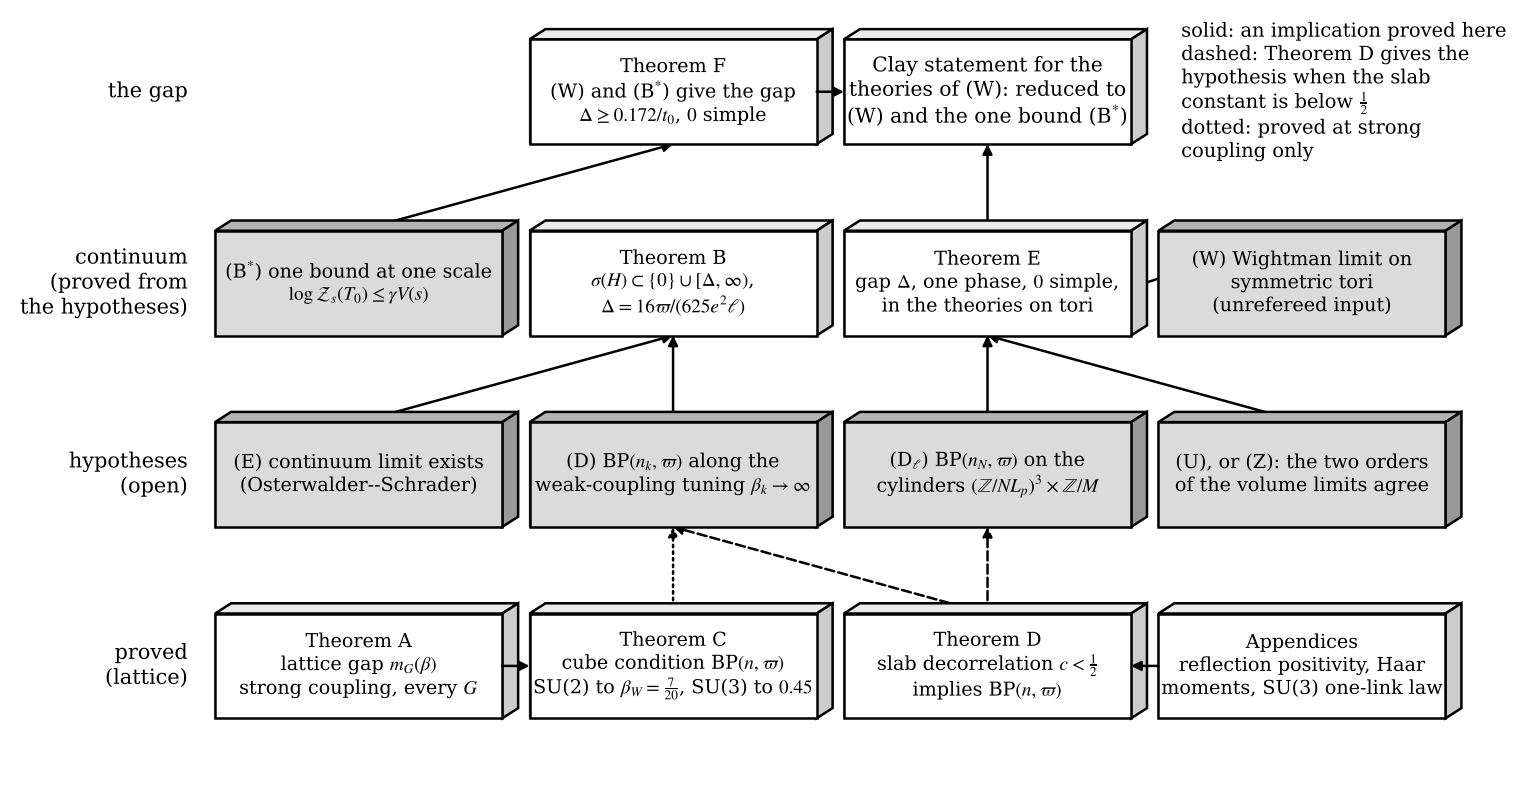
\includegraphics[width=\textwidth]{figures/fig_roadmap.png}
\caption{The logical structure of the paper. White boxes are theorems proved here, grey boxes are hypotheses; solid arrows are implications proved here, the dashed arrows are Theorem~\ref{thm:D}, which yields the cube condition when the slab decorrelation constant is below $\frac12$ (on cylinders by Corollary~\ref{cor:cylinders}), and the dotted arrow records that Theorem~\ref{thm:C} proves the cube condition at strong coupling only. With the construction of~\cite{OAI26} as the existence input (W), the statement of the Clay problem for its theories reduces to (Z) or (U), and to (D$_\ell$) or the slab decorrelation (Theorem~E), and all of these follow from the single bound (B$^{*}$) at one scale (Theorem~F).}
\label{fig:roadmap}
\end{figure}

\subsection{Related work}

Strong-coupling clustering goes back to Osterwalder and Seiler \cite{OSei78}
and Seiler \cite{Sei82}; probabilistic treatments include the survey of
Chatterjee \cite{Chat19}, the Langevin approach of Shen, Zhu and Zhu
\cite{SZZ23}, whose Bakry--\'Emery argument we sharpen, and correlation
decay for finite gauge groups at weak coupling by Adhikari and Cao \cite{AC25}.
In two dimensions the continuum measure is known
\cite{GKS89,Dri89,Lev03}. The transfer matrix of lattice gauge theory is
L\"uscher's \cite{Lus77}, with the temporal gauge and the positivity of the
transfer matrix in Creutz's form~\cite{Cre77}, and the Osterwalder--Schrader reconstruction on the
lattice is due to Osterwalder and Seiler \cite{OSei78}. 
One of us (I.~J.~S.) has formalised in Lean~4 with Mathlib, in a separate
development, without
unproved statements and with only the standard axioms, several ingredients of
the strong-coupling analysis on periodic lattices: the Haar probability on
$\SU(N)$, an infinite-volume Gibbs state obtained as a limit of torus states,
site reflection positivity and the transfer matrix, the Holley--Stroock~\cite{HS87}
comparison, Dobrushin's covariance bounds, and the passage from decay of
correlations to a transfer-matrix gap (one direction of
Proposition~\ref{prop:gapdecay}). For the periodic state it proves a
transfer-matrix gap for every $N$ at $\beta_W<5.9\cdot10^{-5}$, and explicit
single-link heat-bath gaps on boxes of side fifteen for $\SU(2)$ at
$\beta_W\le0.166$ and for $\SU(3)$ at $\beta_W\le0.38$ (the coupling there is
$\beta_W/2$). It also proves, by a Poincar\'e inequality and a light-cone
argument different from Lemma~\ref{lem:speed}, that an ungauged one-cube
influence condition gives a lattice gap of order $1/n$; this is a variant of
the lattice step, Theorem~\ref{thm:decay} and Corollary~\ref{cor:latticegap},
at a smaller rate. The continuum step, the gauge
fixing and the curvature bounds are not part of that development, which shares
with this paper the open hypothesis (D).

